\documentclass[12pt,a4paper]{book}
\raggedbottom


% -------------------------------------------------
% Diseño de capítulos y secciones
% -------------------------------------------------

\usepackage{titlesec}
\usepackage{xcolor}

\definecolor{chapterrule}{gray}{0.55}

\titleformat{\chapter}[hang]
  {\sffamily\bfseries\Large}
  {\thechapter}
  {1em}
  {}
  [\vspace{0.5ex}{\color{chapterrule}\titlerule[0.4pt]}]

\titlespacing*{\chapter}
  {0pt}
  {0pt}
  {2.5ex}

\titleformat{\section}
  {\sffamily\bfseries\normalsize}
  {\thesection}
  {1em}
  {}

\titlespacing*{\section}
  {0pt}
  {2.5ex}
  {1ex}

% -------------------------------------------------

\usepackage{ugmath_notas}
\usepackage{float}
\usepackage{placeins}
\usepackage[labelfont=bf,labelsep=space]{caption}
\usepackage{pdfpages}
\usepackage{tikz-cd}
\usepackage{amsthm}
\renewcommand{\Tr}{\operatorname{Tr}}
\newcommand{\llaves}[1]{\{#1\}}
\newcommand{\parentesis}[1]{\left(#1\right)}
\newcommand{\corchetes}[1]{\left[#1\right]}
\newcommand{\llavesgrande}[1]{\big\{#1\big\}}
\newcommand{\llavesgrandes}[1]{\left\{#1\right\}}
\newcommand{\comillas}[1]{``#1''}


\begin{document}
        
    
    \thispagestyle{empty}
    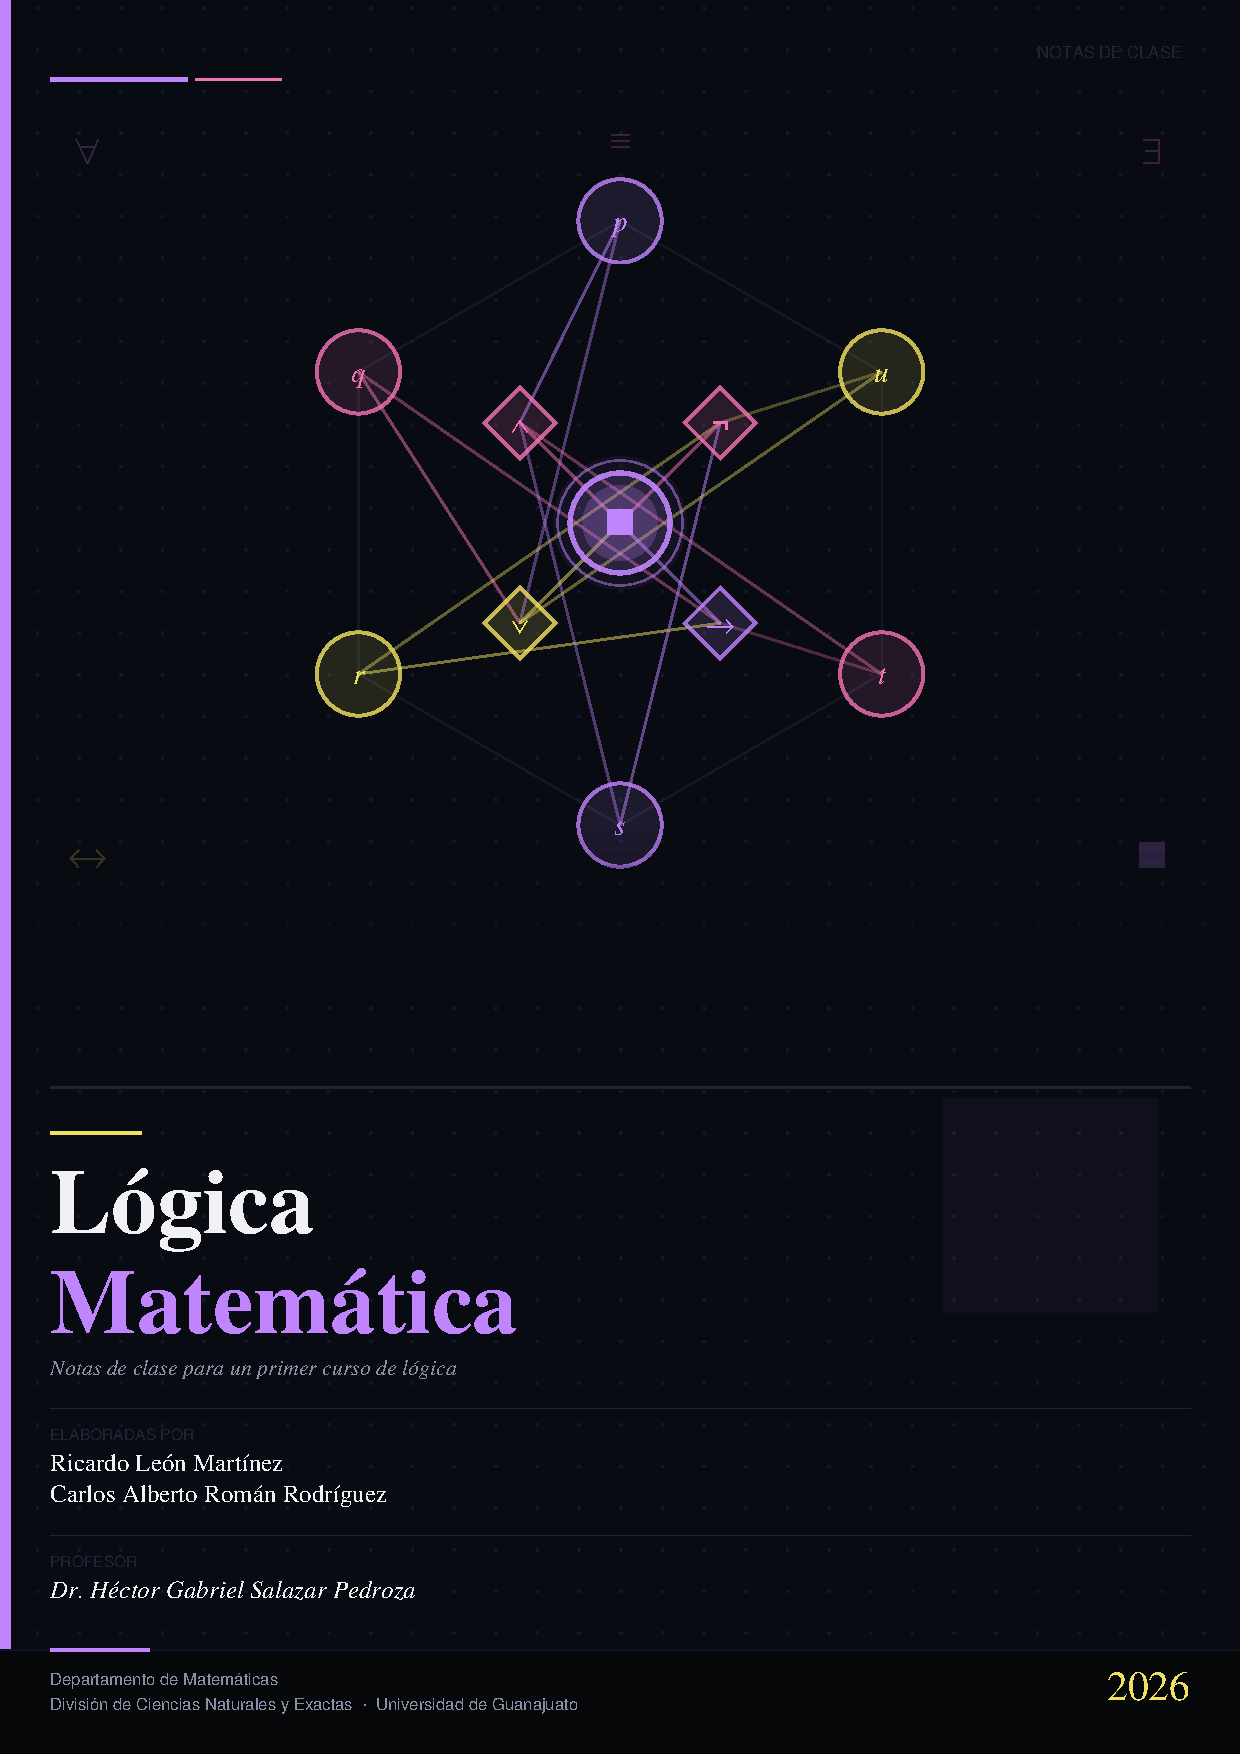
\includepdf[pages=1]{portada_logica_matematica.pdf}

    \begin{flushright}
      \thispagestyle{empty}

        \textbf{Ricardo}\\[0.3cm]
        
        Aqui son las dedicatorias pero hay que ponerlas hasta el final

        \textbf{Roman}
    \end{flushright}

    % ---------------- NOTA DE ERRORES ----------------

    \cleardoublepage
    \thispagestyle{empty}

    \begin{mdframed}[style=mdgreenbox]
        \begin{center}
        \small
        Estas notas fueron elaboradas con fines académicos.\\
        A pesar del cuidado puesto en su redacción,\\
        es posible que existan errores u omisiones.\\[0.3cm]

        Cualquier corrección, sugerencia o comentario será bienvenido
        en los correos correo: \\[0.3cm]

        ricardo.leon@cimat.mx\\
        carlos.roman@cimat.mx
        \end{center}
    \end{mdframed}

    % -------------------------------------------------
    
    \setcounter{page}{1}
    \tableofcontents

    \chapter{Lógica Proposicional}

    \section{¿Que es la lógica proposicional?}

    En lógica proposicional, las formulas atomicas son proposiciones. Cualquier afirmación vale. Por ejemplo

    \begin{quote}
        A=\comillas{Aristóteles ha muerto,}\\
        B=\comillas{Barcelona está a orillas del Sena,} y\\
        C=\comillas{Courtney Love es alta}
    \end{quote}

    son formulas atomicas. Las fórmulas atómicas son los elementos básicos que se utilizan para construir
    proposiciones. En cualquier lógica, una proposición se considera un tipo concreto de formula. En la
    lógica proposicional, no existe distinción entre estos dos términos. Utilizamos \comillas{fórmula} y 
    \comillas{proposición} indistintamente.\\
    En la lógica proposicional, al igual que en todas las lógicas que estudiamos, cada proposición es verdadera
    o falsa. A la proposición se le asigna, en consecuencia, un \textit{valor de verdad} de 1 o 0. En el ejemplo anterior, podemos
    asignar el valor de verdad 1 a la fórmula A y el valor de verdad 0 a la fórmula B. Si tomamos la proposición C al pie de la letra,
    su veracidad es discutible. Quiza, tendría mas sentido permitir valores de verdad entre 0 y 1. Podriamos asignar un 0,75 a la afirmación C
    si la señorita Love es mas alta que el $75\%$ de las mujeres estadounidenses. La lógica difusa permite tales valores de verdad,
    pero las lógicas clásicas que estudiamos no.\\
    De hecho, el contenido de las proposiciones no es relevante para la lógica proposicional. De ahora en adelante, las fórmulas
    atómicas se denotarán únicamente mediante las letras mayúsculas A, B, C,$\dots$ (posiblemente con subíndices) sin hacer referencia a lo
    que estas proposiciones realmente dicen. La veracidad de estas fórmulas no nos concierne. La lógica proposicional no es el estudio de la verdad,
    sino de la relación entre la verdad de una afirmación y la de otra.\\
    El lenguaje de la lógica proposicional contiene palabras como \comillas{no}, \comillas{y}, \comillas{o}, \comillas{implica} y
    \comillas{si y solo si}. Estas palabras se representan mediante símbolos:

    \begin{gather*}
        \neg\text{ para \comillas{no}, }\land\text{ para \comillas{y}, }\lor\text{ para \comillas{o},}\\
        \rightarrow\text{ para \comillas{implica}, }\leftrightarrow\text{ para \comillas{si y solo si}.}
    \end{gather*}

    Como ocurre siempre que se traduce de un idioma a otro, esta correspondencia no es exacta. A diferencia de sus equivalentes en inglés,
    estos simbolos representan conceptos precisos e invariables. El significado de una palabra en inglés, por el contrario, siempre depende
    del contexto. Por ejemplo, $\wedge$ representa un concepto similar, pero no idéntico, a \comillas{y}. Para las fórmulas atómicas
    $A$, $B$ y $A\wedge B$ siempre significa los mismo que $B\wedge A$. Esto no siempre es así con la palabra \comillas{y}. La oración

    \begin{quote}
        Se puso muy enferma y fue al médico.
    \end{quote}

    no tiene el mismo significado que

    \begin{quote}
        Fue al médico y se puso muy mal.
    \end{quote}

    Del mismo modo, $\vee$ difiere de \comillas{o}. En el lenguaje coloquial, el uso de \comillas{A o B} suele excluir la posibilidad
    de que se den tanto A como B. En lógica proposicional, $A\vee B$ siempre significa o bien $A$, o bien $B$, o bien tanto $A$
    como $B$.\\
    Debemos definir con precisión los símbolos $\neg,\wedge,\vee,\rightarrow\text{ y }\ssi$. Nos enfrentamos
    al dilema de cómo definir la primera de un lenguaje (¡sin recurrir a ninguna otra palabra!). Por este motivo,
    tomamos los simbolos $\neg$ y $\wedge$ como \textit{primitivos}. Definimos los demás símbolos en función de
    estos dos. Aunque no definimos $\neg$ y $\wedge$ en función de los demás símbolos, sí describimos la semántica
    de estos símbolos de forma inequívoca.\\
    Antes de describir la semántica del lenguaje, abordaremos la sintaxis. Mientras que la semántica se ocupa del significado, o interepretación,
    de las oraciones en el lenguaje, la sintaxis se ocupa de la gramática del lenguaje. La sintaxis de la lógica proposicional nos indica
    qué cadenas de símbolos son admisibles como fórmulas. Naturalmente, cualquier fórmula atómica es una fórmula. Además, contamos con las dos
    reglas siguientes.

    \begin{quote}
        (R1) Si $F$ es una fórmula, entonces $\neg F$ es una fórmula.\\
        (R2) Si $F$ y $G$ son fórmulas, entonces $(F\wedge G)$ es una fórmula.
    \end{quote}

    \begin{definicion}[Negación y conjunción]
        La fórmula $\neg F$ es la negación de $F$ y la fórmula $(F\wedge G)$ es la conjunción de $F$ y $G$.
    \end{definicion}

    \begin{definicion}
        Una cadena finita de símbolos es una fórmula de la lógica proposicional si y solo si se construye a partir de fórmulas atómicas
        mediante la aplicación de las reglas (R1) y (R2).
    \end{definicion}

    \begin{ejemplo}
        $\neg(\neg(A\wedge B)\wedge\neg C)$ es una fórmula, mientras que $((A\neg\wedge)B(C\neg$ no lo es.
    \end{ejemplo}

    Obsérvese que hemos restringido la definición de fórmula a los símbolos primitivos $\neg$ y $\wedge$. Si tuvieramos que escribir
    la sintaxis de la lógica proposicional a un ordenador, esta definición de fórmula sería suficiente. Sin embargo, para que las fórmulas
    resulten mas comprensibles para los humanos, incluimos los demás símbolos ($\vee,$ $\rightarrow,$ y $\ssi$) que se definirán mas adelante.
    Podemos considerar las fórmulas que incluyen estos símbolos como abreviaturas de fórmulas más complicadas que solo contienen 
    $\neg$ y $\wedge$. La inclusión de estos símbolos hace que las fórmulas sean más fáciles de leer (para nosotros, los humanos).



\end{document}